\begin{sidewaysfigure}
  \centering
  \vspace{0.65\textwidth}
  \begin{minipage}{.7\textwidth} % adjust the width as needed

    \begin{minipage}{\textwidth}
      \centering
      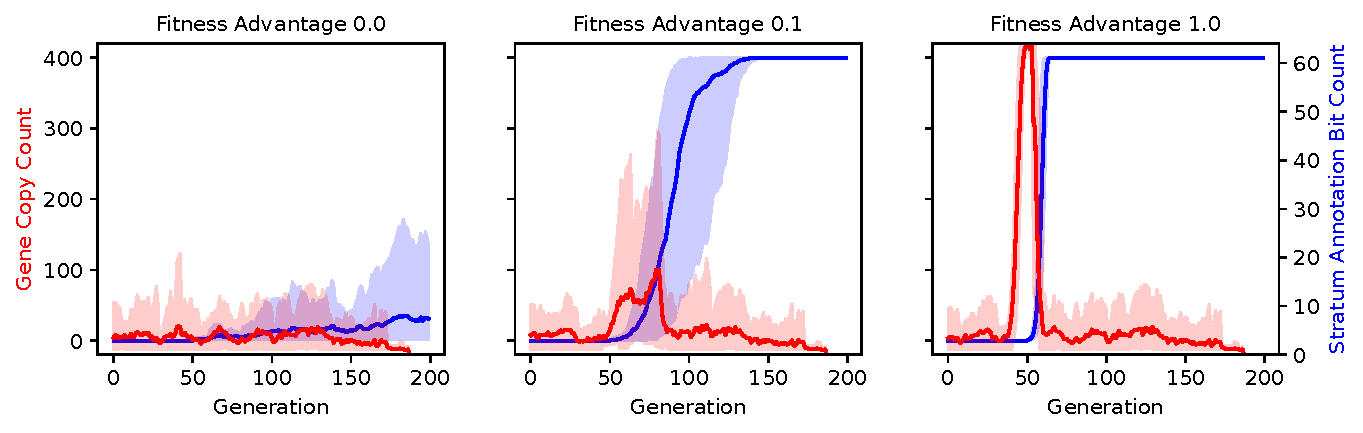
\includegraphics[width=\textwidth]{notebooks/notebooks/teeplots/col=fitness-advantage+viz=facet-lineplot-twiny+x=generation+y1=prevalence+y2=annotation+ext=}
      \subcaption{Cross-replicate aggregate, shaded bands are 95 percentile intervals}
      \label{fig:selection-example-replicates:aggregate}
    \end{minipage}

    \vspace{1cm}

    \centering
    \begin{minipage}{0.32\textwidth}
      \centering
      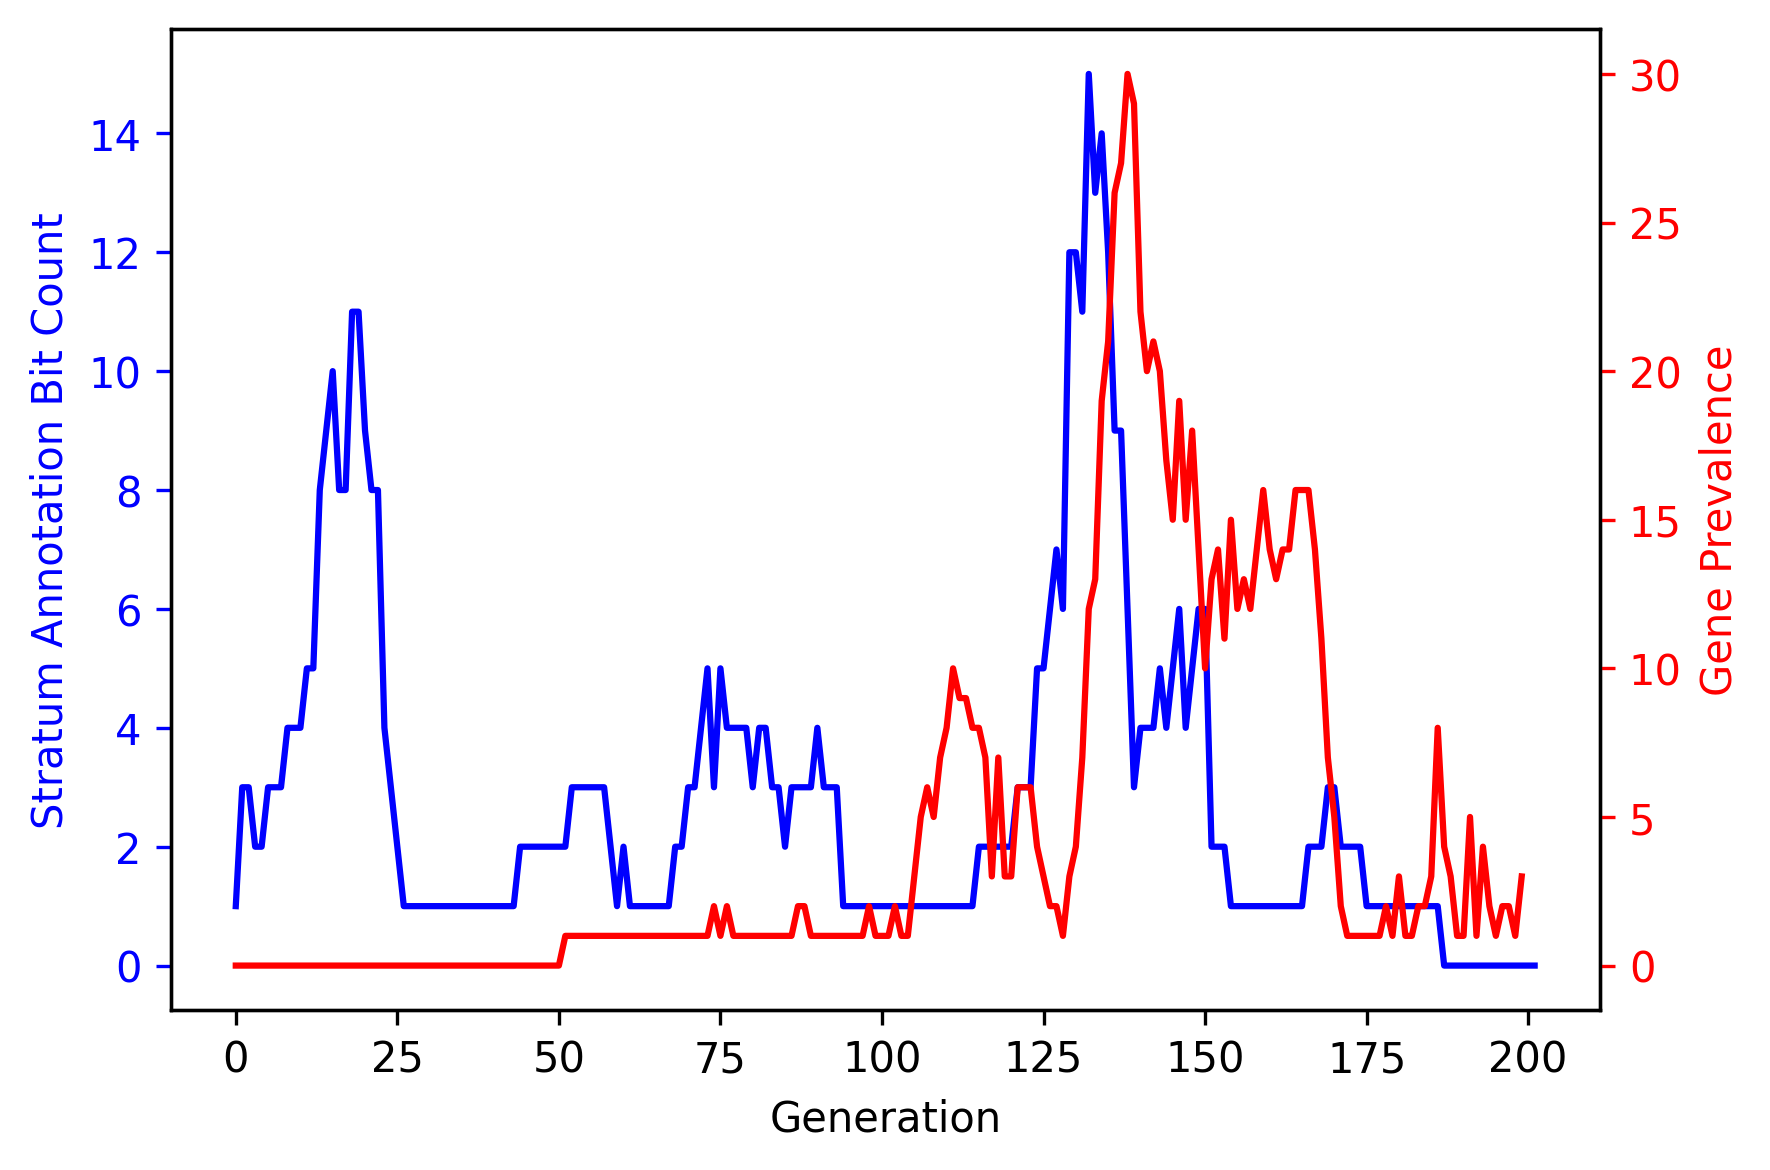
\includegraphics[width=\textwidth]{notebooks/notebooks/teeplots/fitness-advantage=0.0+notebook=gene-selection-inference+replicate=0+viz=plot-sweep-and-annotations+ext=}
      \subcaption{Example replicate with fitness advantage 0.0}
      \label{fig:selection-example-replicates:fit-0-0}
    \end{minipage}
    \begin{minipage}{0.32\textwidth}
      \centering
      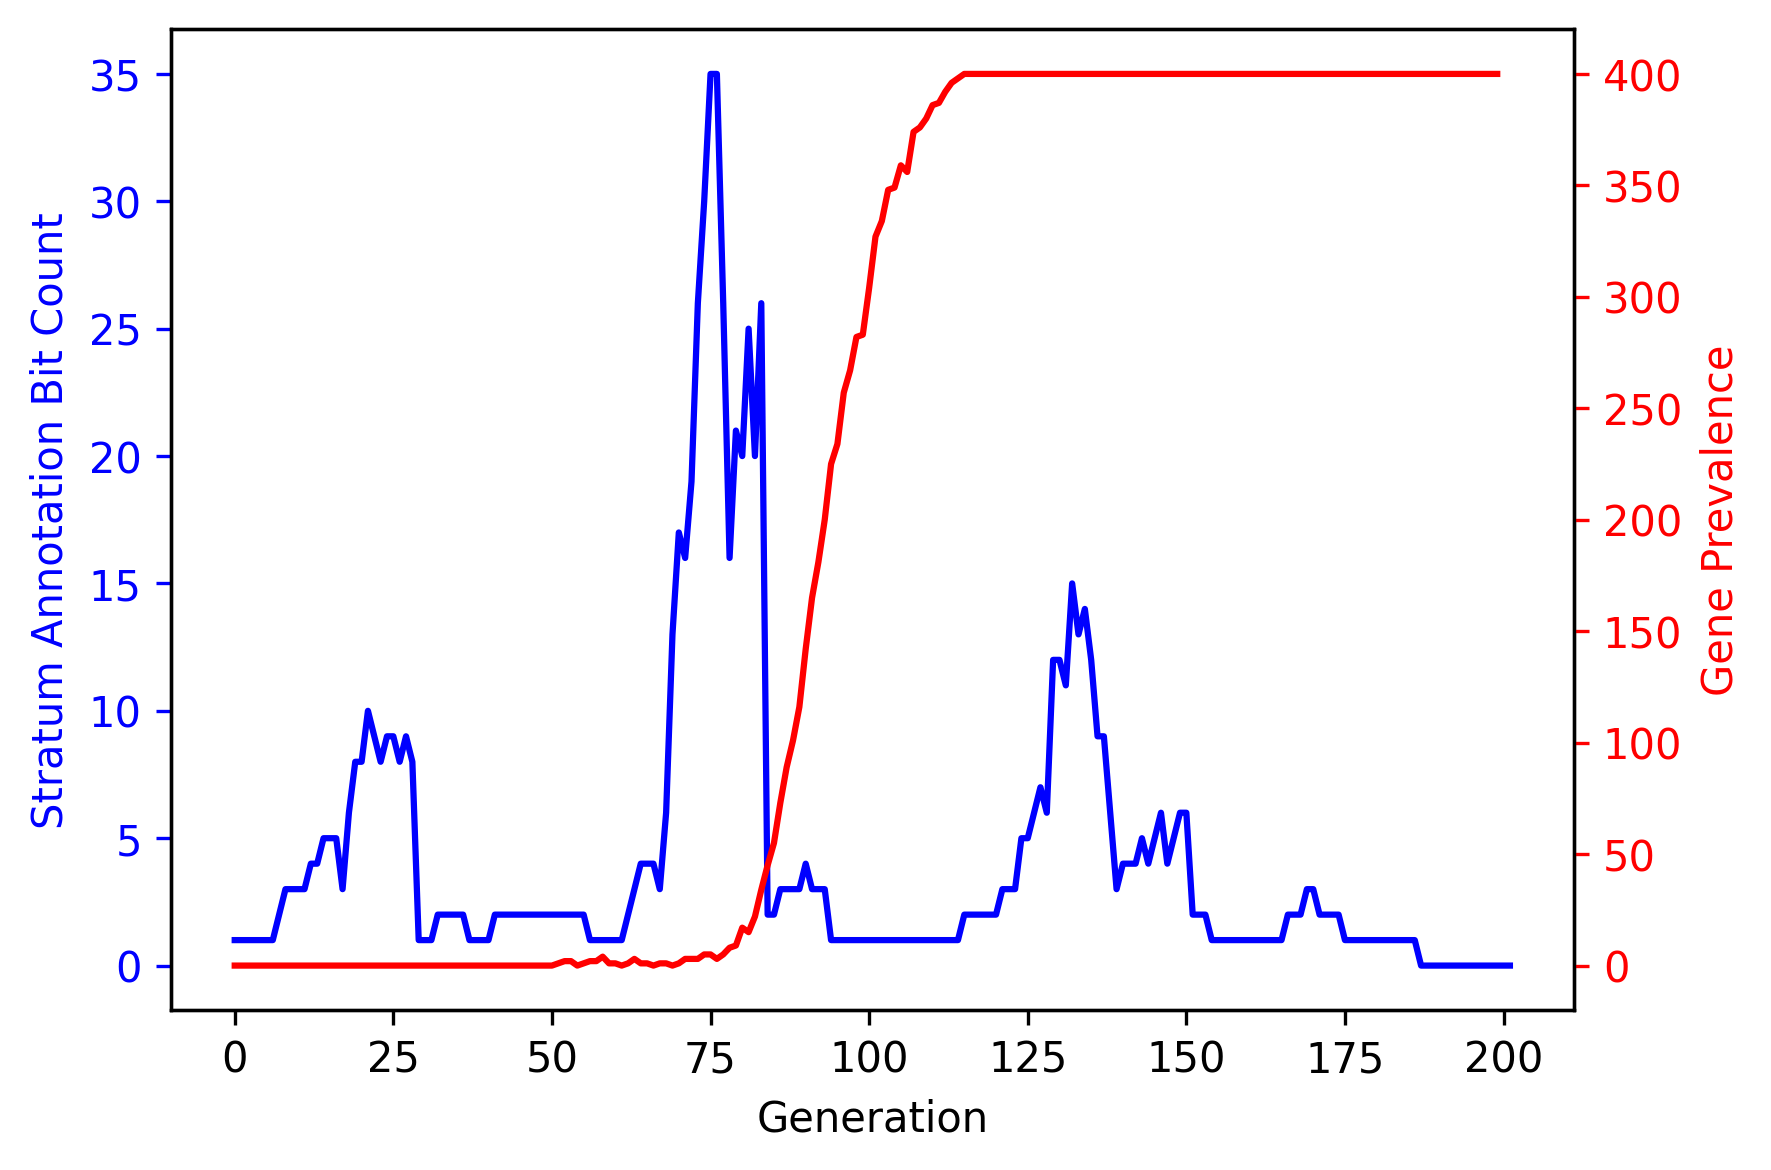
\includegraphics[width=\textwidth]{notebooks/notebooks/teeplots/fitness-advantage=0.1+notebook=gene-selection-inference+replicate=0+viz=plot-sweep-and-annotations+ext=}
      \subcaption{Example replicate with fitness advantage 0.1}
      \label{fig:selection-example-replicates:fit-0-1}
    \end{minipage}
    \begin{minipage}{0.32\textwidth}
      \centering
      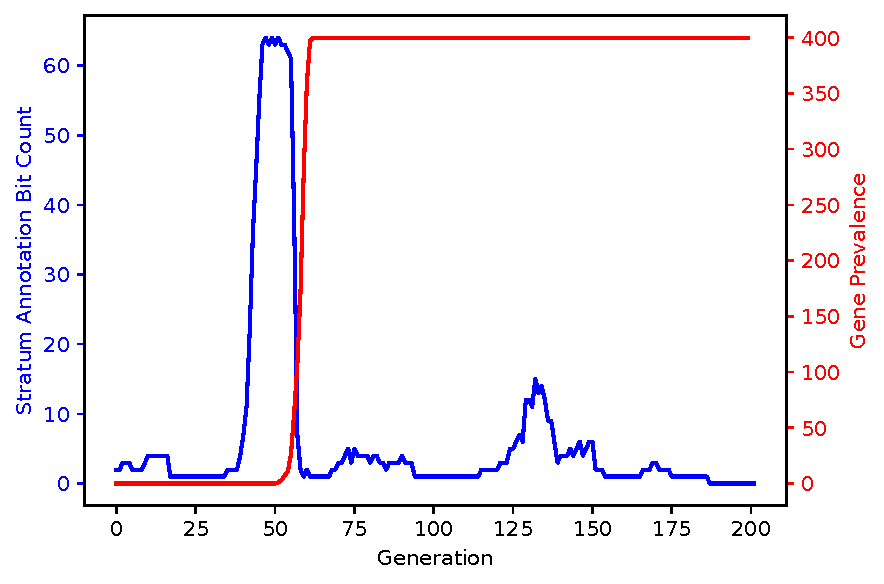
\includegraphics[width=\textwidth]{notebooks/notebooks/teeplots/fitness-advantage=1.0+notebook=gene-selection-inference+replicate=0+viz=plot-sweep-and-annotations+ext=}
      \subcaption{Example replicate with fitness advantage 1.0}
      \label{fig:selection-example-replicates:fit-1-0}
    \end{minipage}%


  \end{minipage}
  \hfill % Creates horizontal space. Can also use \hspace{<len>}
  \begin{minipage}{.25\textwidth} % adjust the width as needed
    \caption{
    Gene prevalence trajectories (shown in red) and 16-generation rolling sums of gene prevalence annotation bit counts (shown in blue) across generations by selection strength treatment.
    Top row summarizes distribution across replicates.
    Bottom row shows an example replicate of each treatment.
    Fitness advantage 0.0 inferred no selective benefit, so all selection detections on this treatment are false positives.
    Fitness advantage 0.1 experienced relatively weak selection and fitness advantage 1.0 experienced strong selection.
    Spikes of high gene prevalence annotation bit count (blue) are indicative of selective dynamics.
    Selection is detected for a replicate if any 16-generation rolling sum of gene prevalence annotation bit count (Section \ref{sec:dist-gene-prevalence-est}) exceeds the threshold.
    Note that $y$ axis scaling differs among bottom-row graphs.
    }
    \label{fig:selection-example-replicates}
  \end{minipage}

\end{sidewaysfigure}
